%
% section 6.2
%
\section{Υπηρεσίες Διαδικτύου}

Οι υπηρεσίες του Διαδικτύου και πολλές εφαρμογές λογισμικού στηρίζονται στο μοντέλο \emph{Πελάτη -- Εξυπηρετητή}. Στο μοντέλο αυτό ο Εξυπηρετητής οργανώνει και διαχειρίζεται το αρχείο δεδομένων ενώ δέχεται αιτήματα και απαντά στο πρόγραμμα Πελάτης. Το πρόγραμμα Πελάτης θέτει ερωτήματα στον εξυπηρετητή και αποκωδικοποιεί τις απαντήσεις του εξυπηρετητή. 

 \begin{figure}[!ht]
  \centering
  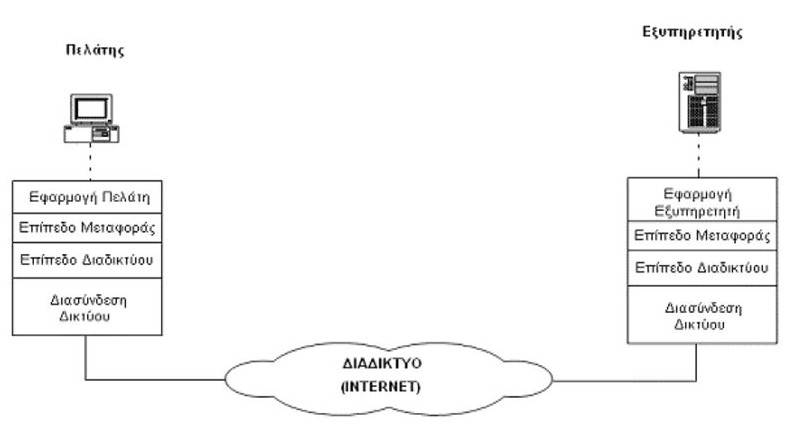
\includegraphics[width=0.85\textwidth]{images/chapter6/6-5}
  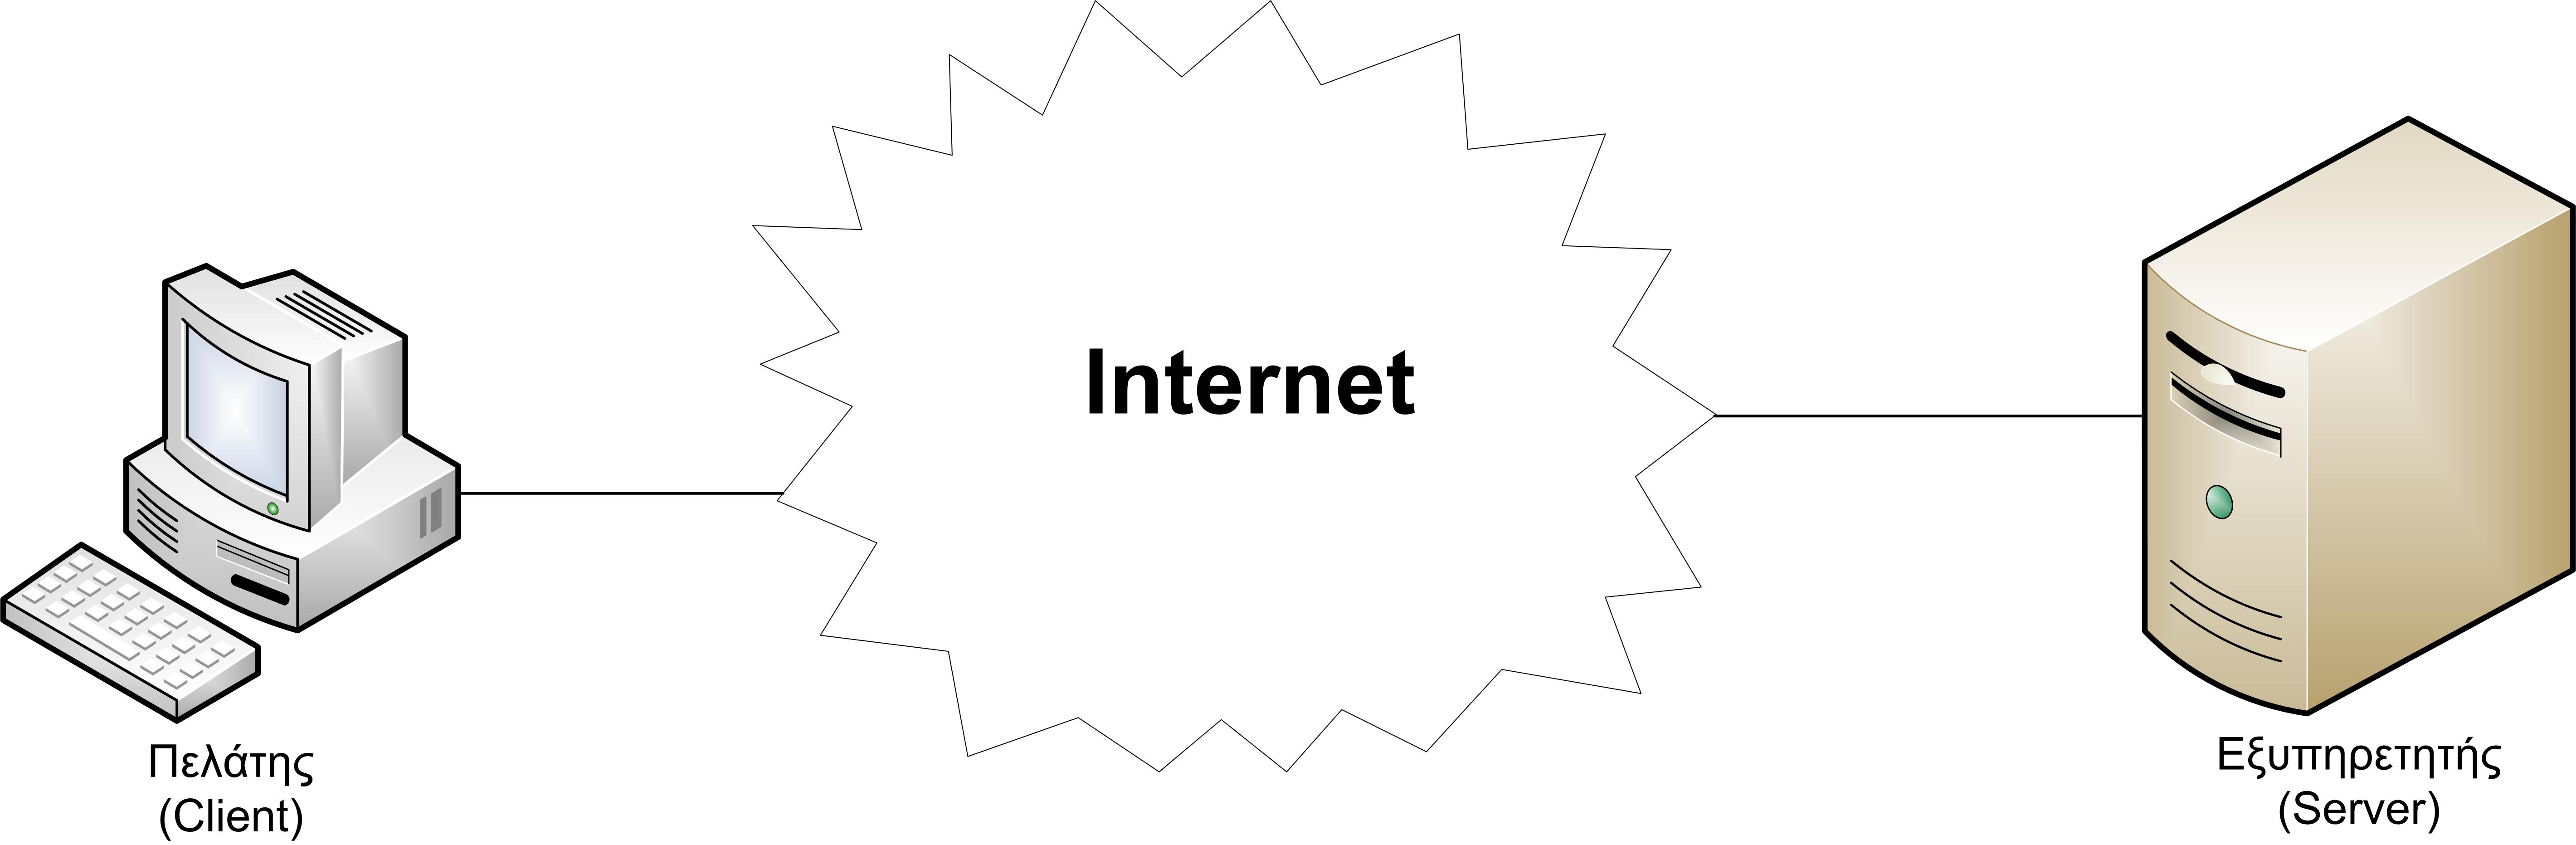
\includegraphics[width=0.85\textwidth]{images/chapter6/6-6}
  \caption {\textsl{Μοντέλο Πελάτη -- Εξυπηρετητή στο TCP/IP και στην Υπηρεσία Ιστοσελίδων }}
  \label{6-5}
\end{figure}

Το μοντέλο Πελάτη -- Εξυπηρετητή υλοποιείται με δύο ανεξάρτητα τμήματα λογισμικού:

\begin{itemize}
\item Το πρόγραμμα του \textbf{Εξυπηρετητή (Server)} εγκαθίσταται σε ένα ή περισσότερους υπολογιστές. Ένας εξυπηρετητής μπορεί συνήθως να εξυπηρετήσει ταυτόχρονα εκατοντάδες ή και χιλιάδες Πελάτες
\item Το πρόγραμμα του \textbf{Πελάτη (Client)} εγκαθίσταται σε πολλούς υπολογιστές
\end{itemize}

Για παράδειγμα ένας εξυπηρετητής ιστοσελίδων (σχήμα \ref{6-5}) μιας δικτυακής τοποθεσίας εκτελείται σε ένα μηχάνημα εξυπηρετητή. Ο εξυπηρετητής αυτός διαχειρίζεται τα αρχεία της ιστοσελίδας τα οποία τυπικά βρίσκονται αποθηκευμένα σε ένα κατάλογο (φάκελο) στο σύστημα αρχείων του εξυπηρετητή. Ο εξυπηρετητής ιστοσελίδων δέχεται συνδέσεις από πελάτες μέσω του πρωτοκόλλου TCP (στη θύρα 80). Οι πελάτες με αιτήματα τους ζητούν συγκεκριμένες σελίδες (αρχεία μορφής HTML) και τα στοιχεία τους (εικόνες κλπ) και ο εξυπηρετητής ανταποκρίνεται στέλνοντας απαντήσεις (κείμενο σε μορφή HTML κλπ).  Ένας μόνο εξυπηρετητής μπορεί να ανταποκριθεί ταυτόχρονα σε χιλιάδες πελάτες (ανάλογα και με τη δυναμική του μηχανήματος και της γραμμής). Το πρόγραμμα πελάτης σε αυτή τη περίπτωση είναι ο φυλλομετρητής (browser) που εκτελείται στο μηχάνημα τελικού χρήστη. 